% Created by tikzDevice version 0.11 on 2018-12-11 10:42:26
% !TEX encoding = UTF-8 Unicode
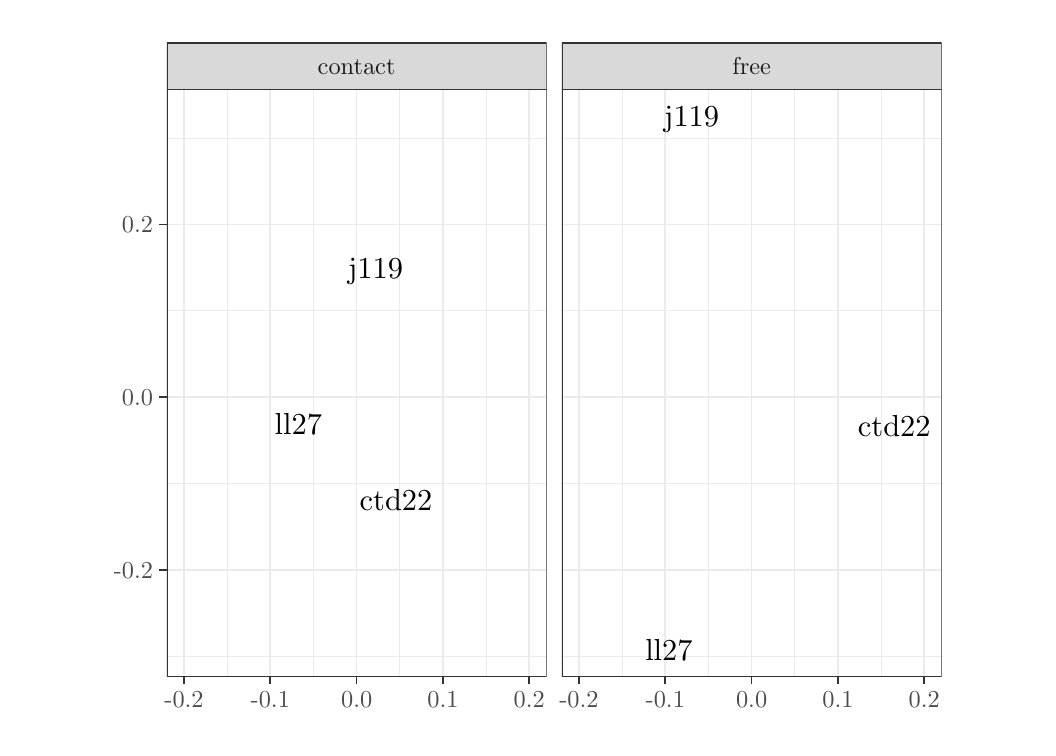
\begin{tikzpicture}[x=1pt,y=1pt]
\definecolor{fillColor}{RGB}{255,255,255}
\path[use as bounding box,fill=fillColor,fill opacity=0.00] (0,0) rectangle (361.35,252.94);
\begin{scope}
\path[clip] ( 25.63,  0.00) rectangle (335.72,252.94);
\definecolor{drawColor}{RGB}{255,255,255}
\definecolor{fillColor}{RGB}{255,255,255}

\path[draw=drawColor,line width= 0.6pt,line join=round,line cap=round,fill=fillColor] ( 25.63,  0.00) rectangle (335.72,252.94);
\end{scope}
\begin{scope}
\path[clip] ( 50.26, 18.45) rectangle (187.49,230.64);
\definecolor{fillColor}{RGB}{255,255,255}

\path[fill=fillColor] ( 50.26, 18.45) rectangle (187.49,230.64);
\definecolor{drawColor}{gray}{0.92}

\path[draw=drawColor,line width= 0.3pt,line join=round] ( 50.26, 25.85) --
	(187.49, 25.85);

\path[draw=drawColor,line width= 0.3pt,line join=round] ( 50.26, 88.23) --
	(187.49, 88.23);

\path[draw=drawColor,line width= 0.3pt,line join=round] ( 50.26,150.61) --
	(187.49,150.61);

\path[draw=drawColor,line width= 0.3pt,line join=round] ( 50.26,212.99) --
	(187.49,212.99);

\path[draw=drawColor,line width= 0.3pt,line join=round] ( 72.09, 18.45) --
	( 72.09,230.64);

\path[draw=drawColor,line width= 0.3pt,line join=round] (103.28, 18.45) --
	(103.28,230.64);

\path[draw=drawColor,line width= 0.3pt,line join=round] (134.47, 18.45) --
	(134.47,230.64);

\path[draw=drawColor,line width= 0.3pt,line join=round] (165.66, 18.45) --
	(165.66,230.64);

\path[draw=drawColor,line width= 0.6pt,line join=round] ( 50.26, 57.04) --
	(187.49, 57.04);

\path[draw=drawColor,line width= 0.6pt,line join=round] ( 50.26,119.42) --
	(187.49,119.42);

\path[draw=drawColor,line width= 0.6pt,line join=round] ( 50.26,181.80) --
	(187.49,181.80);

\path[draw=drawColor,line width= 0.6pt,line join=round] ( 56.50, 18.45) --
	( 56.50,230.64);

\path[draw=drawColor,line width= 0.6pt,line join=round] ( 87.68, 18.45) --
	( 87.68,230.64);

\path[draw=drawColor,line width= 0.6pt,line join=round] (118.87, 18.45) --
	(118.87,230.64);

\path[draw=drawColor,line width= 0.6pt,line join=round] (150.06, 18.45) --
	(150.06,230.64);

\path[draw=drawColor,line width= 0.6pt,line join=round] (181.25, 18.45) --
	(181.25,230.64);
\definecolor{drawColor}{RGB}{0,0,0}

\node[text=drawColor,anchor=base,inner sep=0pt, outer sep=0pt, scale=  1.10] at (125.71,162.42) {\gls{j119}};

\node[text=drawColor,anchor=base,inner sep=0pt, outer sep=0pt, scale=  1.10] at ( 97.80,105.80) {\gls{ll27}};

\node[text=drawColor,anchor=base,inner sep=0pt, outer sep=0pt, scale=  1.10] at (133.11, 78.64) {\gls{ctd22}};
\definecolor{drawColor}{gray}{0.20}

\path[draw=drawColor,line width= 0.6pt,line join=round,line cap=round] ( 50.26, 18.45) rectangle (187.49,230.64);
\end{scope}
\begin{scope}
\path[clip] (192.99, 18.45) rectangle (330.22,230.64);
\definecolor{fillColor}{RGB}{255,255,255}

\path[fill=fillColor] (192.99, 18.45) rectangle (330.22,230.64);
\definecolor{drawColor}{gray}{0.92}

\path[draw=drawColor,line width= 0.3pt,line join=round] (192.99, 25.85) --
	(330.22, 25.85);

\path[draw=drawColor,line width= 0.3pt,line join=round] (192.99, 88.23) --
	(330.22, 88.23);

\path[draw=drawColor,line width= 0.3pt,line join=round] (192.99,150.61) --
	(330.22,150.61);

\path[draw=drawColor,line width= 0.3pt,line join=round] (192.99,212.99) --
	(330.22,212.99);

\path[draw=drawColor,line width= 0.3pt,line join=round] (214.82, 18.45) --
	(214.82,230.64);

\path[draw=drawColor,line width= 0.3pt,line join=round] (246.01, 18.45) --
	(246.01,230.64);

\path[draw=drawColor,line width= 0.3pt,line join=round] (277.20, 18.45) --
	(277.20,230.64);

\path[draw=drawColor,line width= 0.3pt,line join=round] (308.38, 18.45) --
	(308.38,230.64);

\path[draw=drawColor,line width= 0.6pt,line join=round] (192.99, 57.04) --
	(330.22, 57.04);

\path[draw=drawColor,line width= 0.6pt,line join=round] (192.99,119.42) --
	(330.22,119.42);

\path[draw=drawColor,line width= 0.6pt,line join=round] (192.99,181.80) --
	(330.22,181.80);

\path[draw=drawColor,line width= 0.6pt,line join=round] (199.22, 18.45) --
	(199.22,230.64);

\path[draw=drawColor,line width= 0.6pt,line join=round] (230.41, 18.45) --
	(230.41,230.64);

\path[draw=drawColor,line width= 0.6pt,line join=round] (261.60, 18.45) --
	(261.60,230.64);

\path[draw=drawColor,line width= 0.6pt,line join=round] (292.79, 18.45) --
	(292.79,230.64);

\path[draw=drawColor,line width= 0.6pt,line join=round] (323.98, 18.45) --
	(323.98,230.64);
\definecolor{drawColor}{RGB}{0,0,0}

\node[text=drawColor,anchor=base,inner sep=0pt, outer sep=0pt, scale=  1.10] at (239.94,217.19) {\gls{j119}};

\node[text=drawColor,anchor=base,inner sep=0pt, outer sep=0pt, scale=  1.10] at (231.72, 24.30) {\gls{ll27}};

\node[text=drawColor,anchor=base,inner sep=0pt, outer sep=0pt, scale=  1.10] at (313.15,105.36) {\gls{ctd22}};
\definecolor{drawColor}{gray}{0.20}

\path[draw=drawColor,line width= 0.6pt,line join=round,line cap=round] (192.99, 18.45) rectangle (330.22,230.64);
\end{scope}
\begin{scope}
\path[clip] ( 50.26,230.64) rectangle (187.49,247.45);
\definecolor{drawColor}{gray}{0.20}
\definecolor{fillColor}{gray}{0.85}

\path[draw=drawColor,line width= 0.6pt,line join=round,line cap=round,fill=fillColor] ( 50.26,230.64) rectangle (187.49,247.44);
\definecolor{drawColor}{gray}{0.10}

\node[text=drawColor,anchor=base,inner sep=0pt, outer sep=0pt, scale=  0.88] at (118.87,236.01) {contact};
\end{scope}
\begin{scope}
\path[clip] (192.99,230.64) rectangle (330.22,247.45);
\definecolor{drawColor}{gray}{0.20}
\definecolor{fillColor}{gray}{0.85}

\path[draw=drawColor,line width= 0.6pt,line join=round,line cap=round,fill=fillColor] (192.99,230.64) rectangle (330.22,247.44);
\definecolor{drawColor}{gray}{0.10}

\node[text=drawColor,anchor=base,inner sep=0pt, outer sep=0pt, scale=  0.88] at (261.60,236.01) {free};
\end{scope}
\begin{scope}
\path[clip] (  0.00,  0.00) rectangle (361.35,252.94);
\definecolor{drawColor}{gray}{0.20}

\path[draw=drawColor,line width= 0.6pt,line join=round] ( 56.50, 15.70) --
	( 56.50, 18.45);

\path[draw=drawColor,line width= 0.6pt,line join=round] ( 87.68, 15.70) --
	( 87.68, 18.45);

\path[draw=drawColor,line width= 0.6pt,line join=round] (118.87, 15.70) --
	(118.87, 18.45);

\path[draw=drawColor,line width= 0.6pt,line join=round] (150.06, 15.70) --
	(150.06, 18.45);

\path[draw=drawColor,line width= 0.6pt,line join=round] (181.25, 15.70) --
	(181.25, 18.45);
\end{scope}
\begin{scope}
\path[clip] (  0.00,  0.00) rectangle (361.35,252.94);
\definecolor{drawColor}{gray}{0.30}

\node[text=drawColor,anchor=base,inner sep=0pt, outer sep=0pt, scale=  0.88] at ( 56.50,  7.44) {-0.2};

\node[text=drawColor,anchor=base,inner sep=0pt, outer sep=0pt, scale=  0.88] at ( 87.68,  7.44) {-0.1};

\node[text=drawColor,anchor=base,inner sep=0pt, outer sep=0pt, scale=  0.88] at (118.87,  7.44) {0.0};

\node[text=drawColor,anchor=base,inner sep=0pt, outer sep=0pt, scale=  0.88] at (150.06,  7.44) {0.1};

\node[text=drawColor,anchor=base,inner sep=0pt, outer sep=0pt, scale=  0.88] at (181.25,  7.44) {0.2};
\end{scope}
\begin{scope}
\path[clip] (  0.00,  0.00) rectangle (361.35,252.94);
\definecolor{drawColor}{gray}{0.20}

\path[draw=drawColor,line width= 0.6pt,line join=round] (199.22, 15.70) --
	(199.22, 18.45);

\path[draw=drawColor,line width= 0.6pt,line join=round] (230.41, 15.70) --
	(230.41, 18.45);

\path[draw=drawColor,line width= 0.6pt,line join=round] (261.60, 15.70) --
	(261.60, 18.45);

\path[draw=drawColor,line width= 0.6pt,line join=round] (292.79, 15.70) --
	(292.79, 18.45);

\path[draw=drawColor,line width= 0.6pt,line join=round] (323.98, 15.70) --
	(323.98, 18.45);
\end{scope}
\begin{scope}
\path[clip] (  0.00,  0.00) rectangle (361.35,252.94);
\definecolor{drawColor}{gray}{0.30}

\node[text=drawColor,anchor=base,inner sep=0pt, outer sep=0pt, scale=  0.88] at (199.22,  7.44) {-0.2};

\node[text=drawColor,anchor=base,inner sep=0pt, outer sep=0pt, scale=  0.88] at (230.41,  7.44) {-0.1};

\node[text=drawColor,anchor=base,inner sep=0pt, outer sep=0pt, scale=  0.88] at (261.60,  7.44) {0.0};

\node[text=drawColor,anchor=base,inner sep=0pt, outer sep=0pt, scale=  0.88] at (292.79,  7.44) {0.1};

\node[text=drawColor,anchor=base,inner sep=0pt, outer sep=0pt, scale=  0.88] at (323.98,  7.44) {0.2};
\end{scope}
\begin{scope}
\path[clip] (  0.00,  0.00) rectangle (361.35,252.94);
\definecolor{drawColor}{gray}{0.30}

\node[text=drawColor,anchor=base east,inner sep=0pt, outer sep=0pt, scale=  0.88] at ( 45.31, 54.01) {-0.2};

\node[text=drawColor,anchor=base east,inner sep=0pt, outer sep=0pt, scale=  0.88] at ( 45.31,116.39) {0.0};

\node[text=drawColor,anchor=base east,inner sep=0pt, outer sep=0pt, scale=  0.88] at ( 45.31,178.77) {0.2};
\end{scope}
\begin{scope}
\path[clip] (  0.00,  0.00) rectangle (361.35,252.94);
\definecolor{drawColor}{gray}{0.20}

\path[draw=drawColor,line width= 0.6pt,line join=round] ( 47.51, 57.04) --
	( 50.26, 57.04);

\path[draw=drawColor,line width= 0.6pt,line join=round] ( 47.51,119.42) --
	( 50.26,119.42);

\path[draw=drawColor,line width= 0.6pt,line join=round] ( 47.51,181.80) --
	( 50.26,181.80);
\end{scope}
\end{tikzpicture}
